\documentclass[10pt]{beamer}

\usetheme[progressbar=frametitle]{metropolis}
\usepackage{appendixnumberbeamer}
\usepackage{booktabs}
\usepackage[scale=2]{ccicons}
\usepackage{pgfplots}
\usepgfplotslibrary{dateplot}
\usepackage{xspace}
\newcommand{\themename}{\textbf{\textsc{metropolis}}\xspace}

\usepackage{ragged2e}
\usepackage{multirow}


\title{Comunicação entre Robot Operating System - ROS e SoC com FPGA integrado}
\subtitle{Universidade Federal da Bahia\\
            Programa de Pós-Graduação em Engenharia Elétrica}
\date{\today}
\date{Orientador: Prof. Dr. Wagner Luiz Alves de Oliveira\\Coorientador: Prof. Dr. Paulo César Farias}
\author{Autor: Nestor Dias Pereira Neto}
\institute{Salvador, 5 de dezembro de 2022}
\titlegraphic{\hfill
\includegraphics[height=1.85cm]{imagens/logo.png}}


\begin{document}

\maketitle

\begin{frame}{Agenda}
  \setbeamertemplate{section in toc}[sections numbered]
  \tableofcontents[hideallsubsections]
\end{frame}


%=================================================================
% INTRODUÇÃO
%=================================================================
\section{Introdução}

% Slide CONTEXTUALIZAÇÃO I
%-----------------------------------------------------------------
\metroset{titleformat frame=smallcaps}
\begin{frame}{Contextualização}
	\begin{alertblock}{}
    	\begin{itemize}
		\setlength\itemsep{0.7em}
    	\item Projetos em robótica têm exigido maior percepção do ambiente.
    	\item Maior poder de processamento demanda maior consumo de energia.
    	\item FPGAs possuem potencial para melhorar desempenho de sistemas computacionais.
    	\item MACs de alta velocidade, processamento paralelo e baixas frequências de trabalho são comuns em FPGA. 
    	\item O uso do FPGA pode contribuir com ganho de poder de processamento associado ao baixo consumo.
    	\end{itemize}
    \end{alertblock}
 \nocite{LwIP,freertosbook,ROSeffect,PDSfpga,NiosIIbook,ROSfpga}
\end{frame}

% Slide CONTEXTUALIZAÇÃO II
%-----------------------------------------------------------------
\metroset{titleformat frame=smallcaps}
\begin{frame}{Contextualização}
	\begin{alertblock}{}
    	\begin{itemize}%[label=$\bullet$, itemsep=0.3cm]
		\setlength\itemsep{1em}
		\item Apesar de oferecer grande vantagens o FPGA em projetos de robótica é pouco incentivado.
    	\item Atualmente o framework ROS está se consolidando como o padrão na criação de novas plataformas robóticas.
    	\item O ROS é considerado um sistema operacional para robôs.
    	\item Desenvolver uma solução para estabelecer comunicação entre FPGA e o ROS.
    	\end{itemize}
    \end{alertblock}
 \nocite{LwIP,freertosbook,ROSeffect,PDSfpga,NiosIIbook,ROSfpga}
\end{frame}

% Slide PROBLEMA
%-----------------------------------------------------------------
\metroset{titleformat frame=smallcaps}
\begin{frame}[fragile]{Problema}
	\begin{center}
		\textbf{Como estabelecer a comunicação entre o ROS e um sistema de processamento auxiliar embarcado em um FPGA? }
	\end{center}
	\vspace{0.75cm}
	\begin{justify}
		Este problema é o que este trabalho busca resolver, possibilitando assim, o uso de aceleração por hardware através do FPGA no desenvolvimento de novos projetos de robótica.
	\end{justify}
\end{frame}

% Slide JUSTIFICATIVA
%-----------------------------------------------------------------
% \begin{frame}[fragile]{Justificativa}
%     \begin{itemize}
%         \item Nos últimos anos, novas técnicas para construção de robôs têm sido bastante estudadas e a robótica móvel tem recebido grande atenção.
%         \item Busca por maior autonomia, sistemais mais complexos.
%         \item FPGA uma opção para aumento de desempenho computacional, combinado com baixo consumo.
%         \item Poucas pesquisas relacionadas ao tema.
%         \item Reaproveitamento da pesquisa em outros projetos das mais diversas áreas.
%     \end{itemize}
% \end{frame}

% Slide OBJETIVO GERAL
%-----------------------------------------------------------------
\metroset{titleformat frame=smallcaps}
\begin{frame}{Objetivos}
    \begin{alertblock}{Objetivo geral}
		\vspace{0.25cm}
    	\begin{itemize}
    	\item Desenvolver uma solução para estabelecer comunicação entre \textit{Field-Programmable Gate Array - FPGA}, e o \textit{Robot Operating System - ROS}.
    	\end{itemize}
    \end{alertblock}
\end{frame}

% Slide OBJETIVOS ESPECÍFICOS
%-----------------------------------------------------------------
\metroset{titleformat frame=smallcaps}
\begin{frame}{Objetivos}
	\begin{alertblock}{Objetivos específicos}
        \begin{itemize}
        	\item Estudar teoria dos assuntos relevantes ao projeto: Verilog HDL, Embedded Linx,
			Cyclone V, TCP/IP Stack, ROS;
        	\item Estudar conceitos de programação de sockets em liguagem C++;
        	\item Implementar distribuição Embedded Linux para processador ARM embarcado no
			SoC Cyclone V da Intel;
        	\item Implementar distribuição Embedded Linux para processador ARM.
        	\item Estabelecer comunicação entre o ROS e o Cyclone V, através da tecnologia Gigabit
			Ethernet;
        	\item Avaliar o desempenho da rede entre o computador e o protótipo após a inclusão do
			FPGA ao sistema.
        \end{itemize}
	\end{alertblock}
\end{frame}




%=================================================================
% Parte I: Referenciais Teórico
%=================================================================
\section{Parte I: Referenciais Teórico}




%*****************************************************************
% CAPITULO I
%*****************************************************************

% Slide SYSTEM-ON-CHIP
%-----------------------------------------------------------------
\metroset{titleformat frame=smallcaps}
\begin{frame}{Cyclone V SoC-FPGA}
	% \begin{alertblock}{System-on-Chip}
		\vspace{0.1cm}
		\begin{justify}
			SoC é um acrônimo de \textit{System-on-a-Chip} ou apenas \textit{System on Chip}. Um SoC pode combinar diferentes elementos, em diferentes configurações, para formar um sistema completo.
		\end{justify}
		
		\begin{figure}[h]
			%\caption{{\footnotesize SoC genérico}}
			\begin{center}
				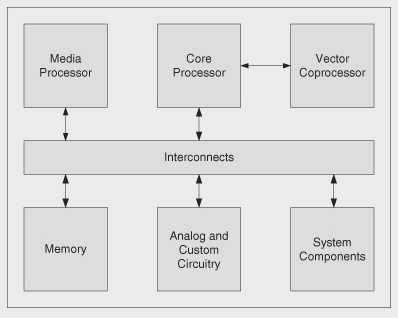
\includegraphics[scale=0.395]{imagens/basicsoc.png}\\
				{\footnotesize \textbf{Fonte:}}
			\end{center}
			\label{fig:SoC}
		\end{figure}
	% \end{alertblock}
\end{frame}

% Slide FAMÍLIA CYCLONE V
%-----------------------------------------------------------------
\metroset{titleformat frame=smallcaps}
\begin{frame}{Cyclone V SoC-FPGA}
	% \begin{alertblock}{Família Cyclone V SoC-FPGA}
		\vspace{0.1cm}
		\begin{justify}
			A Intel fornece uma linha de produtos classificados como SoC-FPGA, os quais se aracterizam por possuir um rede de FPGA integrados a um processador ARM Cortex A9.
		\end{justify}
		\begin{figure}[h]
			%\caption{{\footnotesize SoC genérico}}
			\begin{center}
				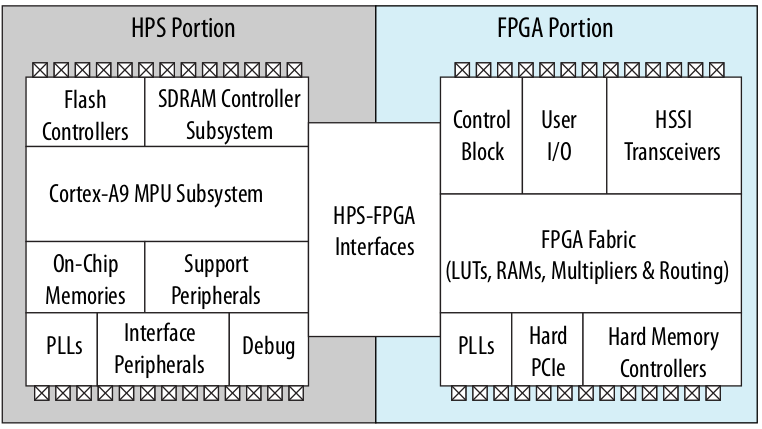
\includegraphics[scale=0.29]{imagens/socfpga.png}\\
				{\footnotesize \textbf{Fonte:}}
			\end{center}
			\label{fig:SoC}
		\end{figure}
	% \end{alertblock}
\end{frame}

% Slide INTERFACES HPS-FPGA
%-----------------------------------------------------------------
\metroset{titleformat frame=smallcaps}
\begin{frame}{Cyclone V SoC-FPGA}
	\begin{alertblock}{}
		\vspace{0.1cm}
		\begin{justify}
			Esta estratégia de interconexão entre o HPS e o FPGA do Cyclone V em um único
			circuito integrado oferece:
		\end{justify}
		\vspace{0.25cm}
		\begin{itemize}
			\setlength\itemsep{1em}
        	\item Largura de banda de pico de mais de 100 Gbps;
        	\item Coerência de dados integrada;
        	\item Significativa economia de energia do sistema, eliminando caminhos de E/S externos
			entre o processador e o FPGA.
        \end{itemize}
	\end{alertblock}
\end{frame}

% Slide PROCESSADOR ARM CORTEX A9
%-----------------------------------------------------------------
\metroset{titleformat frame=smallcaps}
\begin{frame}{Cyclone V SoC-FPGA}
	\begin{alertblock}{Processador ARM Cortex-A9}
		%\vspace{0.1cm}
		\begin{itemize}
			\item É uma linha de processadores ARM de uso geral, otimizados para alcançarem maior desempenho aliado a um baixo consumo.

			\item Possue estrutura interna configuravel, o que oferece flexibilidade ideal para o desenvolvimento de um novo SoC.
		\end{itemize}

		\begin{table}[ht]
			\begin{center}    
				\begin{tabular}{ll}
				\hline
				{\footnotesize Arquitetura}     & {\footnotesize Armv7-A}                     \\ \hline 
				{\footnotesize Multicore}       & {\footnotesize 1-4 cores}                   \\ \hline 
				\multirow{2}{*}{{\footnotesize 
				Suporte ISA}}					& {\footnotesize Extensão DSP}				  \\ \cline{2-2} 
												& {\footnotesize Ponto Flutuante (Opcional)}  \\ \hline 
				{\footnotesize MMU}    			& {\footnotesize Armv7 MMU}       			  \\ \hline 
				\multirow{2}{*}{{\footnotesize 
				Caracteristicas}} 				& \begin{tabular}[c]{@{}l@{}}{\footnotesize 
												  Arquitetura flexisível com caches 
												  configuráveis}\end{tabular}           	  \\ \cline{2-2}
												& \begin{tabular}[c]{@{}l@{}}{\footnotesize 
												  Desempenho 50\% maior do que o Cortex-A8}
												  \end{tabular}   			 				  \\ \hline
				\end{tabular}
				\\
				\vspace{0.2cm}
				{\footnotesize \textbf{Fonte:} }
			\end{center}\label{tab:cortexA9config}
		\end{table}
	\end{alertblock}
\end{frame}

% Slide FPGA
%-----------------------------------------------------------------
\metroset{titleformat frame=smallcaps}
\begin{frame}{Cyclone V SoC-FPGA}
	\begin{alertblock}{Fild-Programmable Gate Array-FPGA}
		\vspace{0.25cm}
		\begin{itemize}
			\setlength\itemsep{1em}
			\item Dispositivos semicondutores construídos através de uma matriz de blocos lógicos configuráveis, os CLBs.
			\item Interconectáveis a partir de conexões Programáveis.
			\item Hardware configuravel pelo usuário.
			\item Poderosas ferramentas de prototipagem.
		\end{itemize}
	\end{alertblock}
\end{frame}

% Slide ARDWARE PROCESSOR SYSTEM I
%-----------------------------------------------------------------
\metroset{titleformat frame=smallcaps}
\begin{frame}{Cyclone V SoC-FPGA}
	\begin{alertblock}{Hardware Processor System}
		\vspace{0.1cm}
		\begin{justify}
			 A família Cyclone V SoC-FPGA é composta por duas partições, uma malha de FPGA e um \textit{Hard Processor System} (HPS). Os principais módulos do HPS são:
		\end{justify}
		\begin{itemize}
			%\setlength\itemsep{0.6em}
			\item \textit{Microprocessador Unit} (MPU), subsistema com um ou dois ARM Cortex-A9.
			\item Controladores de memória Flash.
			\item Controladores de SDRAM.
			\item Sistema de interconexão.
			\item \textit{On-chip memory}.
			\item \textit{Phase-locked loops} (PLLs).
		\end{itemize}
	\end{alertblock}
\end{frame}

% Slide ARDWARE PROCESSOR SYSTEM II
%-----------------------------------------------------------------
\metroset{titleformat frame=smallcaps}
\begin{frame}{Cyclone V SoC-FPGA}
	\begin{alertblock}{Hardware Processor System: FPGA Manager}
		\begin{columns}
			\column{.44\textwidth}
			\begin{alertblock}{}
				\begin{itemize}
					\setlength\itemsep{0.8em}
					\item Configuração do FPGA.
					\item 32 sinais de uso geral.
					\item Status do FPGA.
					\item Interrupções para o HPS a partir do FPGA.
					\item Resetar o FPGA.
				\end{itemize}
			\end{alertblock}
			\column{.66\textwidth}
			\begin{figure}[h]
				%\caption{ROS Master}
				\begin{center}
					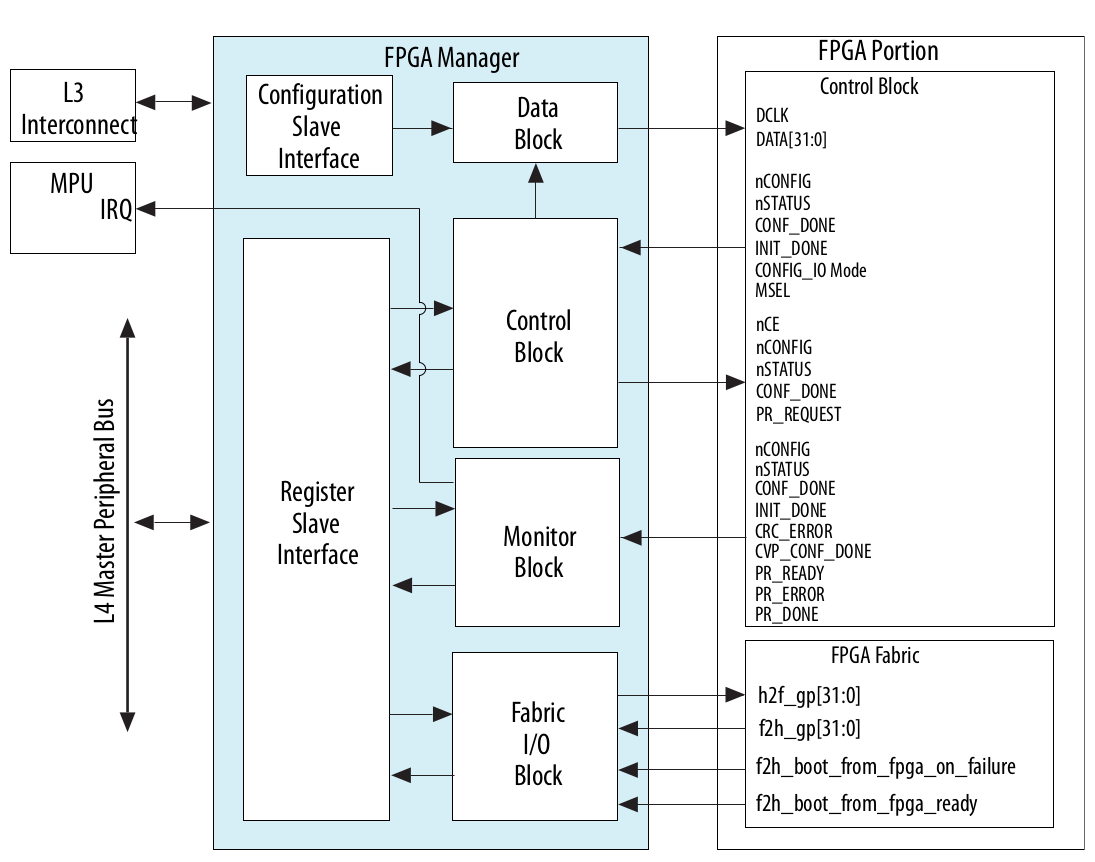
\includegraphics[scale=0.18]{imagens/fpgamanager.png}\\
					{\footnotesize \textbf{Fonte:}}
				\end{center}
				\label{fig:fpgamanager}
			\end{figure}
		\end{columns}
	\end{alertblock}
\end{frame}

% Slide ARDWARE PROCESSOR SYSTEM III
%-----------------------------------------------------------------
\metroset{titleformat frame=smallcaps}
\begin{frame}{Cyclone V SoC-FPGA}
	\begin{alertblock}{Hardware Processor System: HPS-FPGA Bridge}
		\begin{figure}[h]
			%\caption{ROS Master}
			\begin{center}
				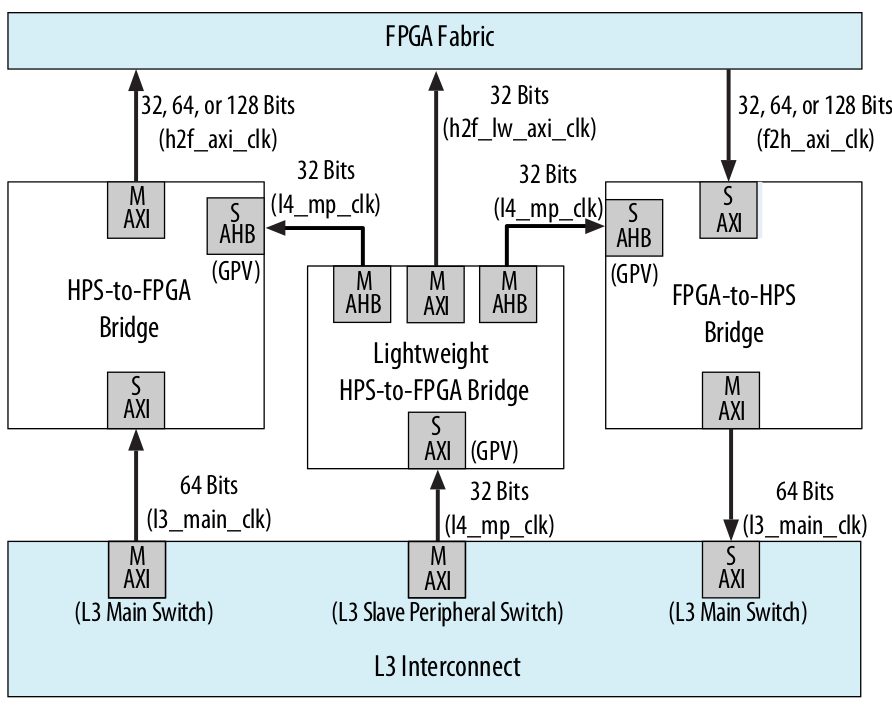
\includegraphics[scale=0.21]{imagens/hps-fpga_bridge.png}\\
				{\footnotesize \textbf{Fonte:}}
			\end{center}
			\label{fig:bridge}
		\end{figure}
	\end{alertblock}
\end{frame}

% Slide ARDWARE PROCESSOR SYSTEM IV
%-----------------------------------------------------------------
\metroset{titleformat frame=smallcaps}
\begin{frame}{Cyclone V SoC-FPGA}
	\begin{alertblock}{Hardware Processor System: Cortex A9 MPU}
		\begin{columns}
			%\hspace{0.1cm}
			\column{.4\textwidth}
			O \textit{Microprocessor Unit Subsystem} (MPU) presentes SoCs da família Cyclone V incluem um Arm Cortex-A9 MPCore, com processador de uso geral de 32 bits com um ou dois núcleos.
			\column{.6\textwidth}
			\begin{figure}[h]
				%\caption{{\footnotesize SoC genérico}}
				\begin{center}
					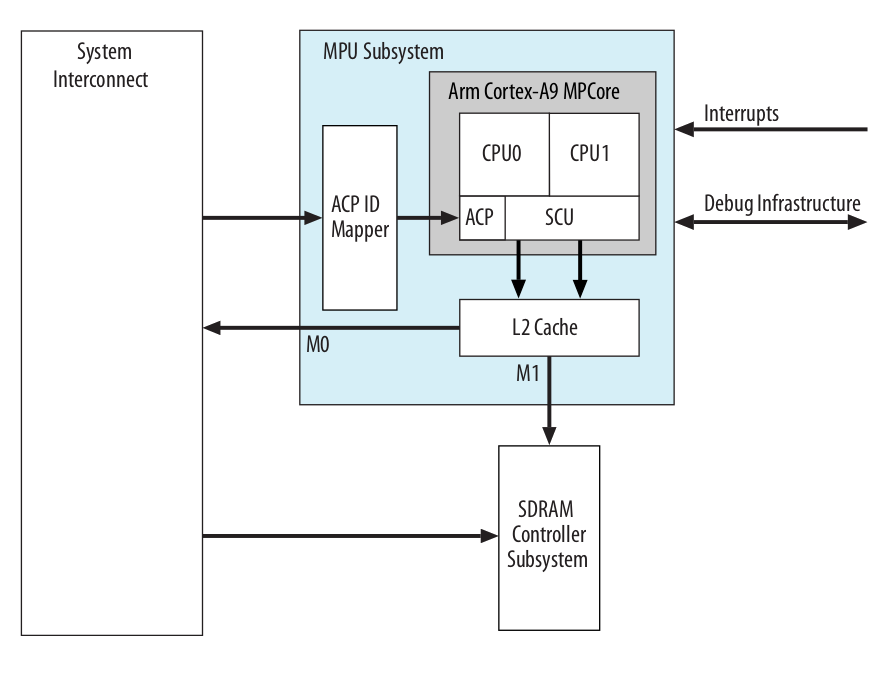
\includegraphics[scale=0.217]{imagens/mpusubsystem.png}\\
					{\footnotesize \textbf{Fonte:}}
				\end{center}
				\label{fig:cycloneV}
			\end{figure}
		\end{columns}
	\end{alertblock}
\end{frame}


% Slide KIT DE DESENVOLVIMENTO
%-----------------------------------------------------------------
\metroset{titleformat frame=smallcaps}
\begin{frame}{Cyclone V SoC-FPGA}
	\begin{alertblock}{Kit de desenvolvimento DE10-nano}
		\begin{figure}[h]
			%\caption{ROS Master}
			\begin{center}
				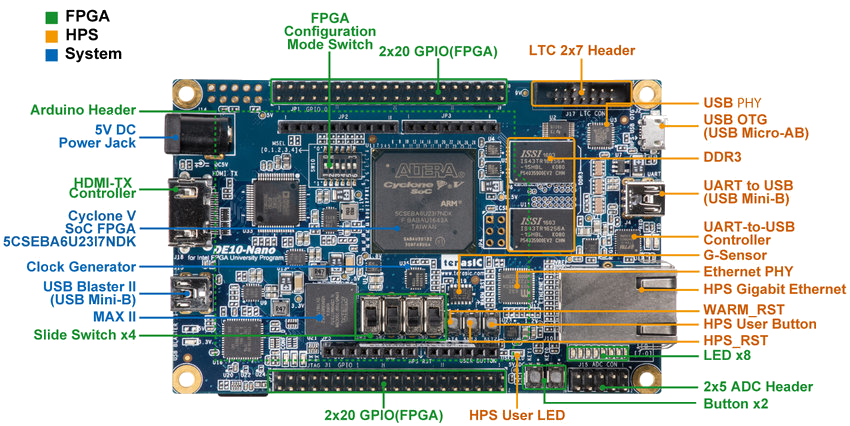
\includegraphics[scale=1.45]{imagens/de10nano.png}\\
				{\footnotesize \textbf{Fonte:}}
			\end{center}
			\label{fig:de10-nano}
		\end{figure}
	\end{alertblock}
\end{frame}
%*****************************************************************
% CAPITULO II
%*****************************************************************

% Slide ROS
%-----------------------------------------------------------------
\metroset{titleformat frame=smallcaps}
\begin{frame}{\textit{Robot Operating System-ROS}}
	\begin{alertblock}{Um sistema operacional para robôs}
		\vspace{0.1cm}
		\begin{justify}
			``O Robot Operating System (ROS) é um conjunto de bibliotecas de software e ferramentas que te auxiliam na construção de aplicações em robótica. De \textit{drivers} ao estado da arte de algoritmos, e com poderosas ferramentas de desenvolvimento, ROS tem o que você precisa para seu próximo projeto de robótica. E tudo é open source'' 
		\end{justify}
		

	\end{alertblock}
\end{frame}

% Slide VANTAGENS ROS
%-----------------------------------------------------------------
\metroset{titleformat frame=smallcaps}
\begin{frame}{\textit{Robot Operating System-ROS}}
	\begin{alertblock}{Vantagens do ROS: Tópico}
		\vspace{0.2cm}
		\begin{itemize}
			\setlength\itemsep{0.7em}
			\item \textbf{Recursos Nativos:} O ROS oferece, de forma nativa, muitos recursos prontos,
			testados e validados pela comunidade.
			\item \textbf{Ferramentas de desenvolvimento:} O ROS é disponibilizado com uma grande quantidade de ferramentas para debugging, visualização, incluindo ferramentas para simulação.
			\item \textbf{Suporte a sensores e atuadores:} Muitos dos sensores e atuadores usados na robótica já são suportados pelo ROS e o número de dispositivos compatíveis aumenta a cada ano.
			\item \textbf{Múltiplas linguagens:} O framework ROS pode ser programado em algumas linguagens de programação modernas.
		\end{itemize}
	\end{alertblock}
\end{frame}

% Slide SISTEMA DE ARQUIVOS
%-----------------------------------------------------------------
\metroset{titleformat frame=smallcaps}
\begin{frame}{\textit{Robot Operating System-ROS}}
	\begin{alertblock}{Sistema de arquivos ROS}
		\vspace{0.2cm}
		\begin{itemize}
			\setlength\itemsep{0.9em}
			\item \textbf{Pacotes:} Pacotes são a unidade de software principal do ROS.
			\item \textbf{Manifesto do pacote:} O arquivo package.xml é conhecido como manifesto do	pacote, ele fornece os metadados a respeito do pacotes.
			\item \textbf{Arquivo .msg:} É o arquivo de descrição de um tipo de mensagem.
			\item \textbf{Arquivo .srv:} É o arquivo de descrição de um tipo de serviço.
			\item \textbf{Repositórios:} Pacotes ROS são compartilhados usando algum tipo de sistema de	controle de versão, como o git.
		\end{itemize}
	\end{alertblock}
\end{frame}

% Slide COMPONENTES ROS TOPIC
%-----------------------------------------------------------------
\metroset{titleformat frame=smallcaps}
\begin{frame}{\textit{Robot Operating System-ROS}}
	\begin{alertblock}{Componentes ROS: Tópicos ROS}
		\vspace{0.7cm}
		\begin{figure}[h]
			%\caption{ROS Master}
			\begin{center}
				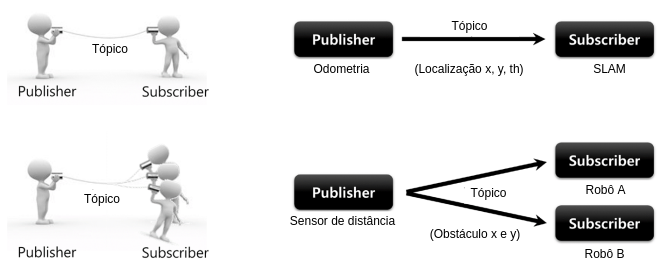
\includegraphics[scale=0.41]{imagens/rostopic.png}\\
				{\footnotesize \textbf{Fonte:}}
			\end{center}
			\label{fig:topico}
		\end{figure}
	\end{alertblock}
\end{frame}

% Slide COMPONENTES ROS MASTER
%-----------------------------------------------------------------
\metroset{titleformat frame=smallcaps}
\begin{frame}{\textit{Robot Operating System-ROS}}
	\begin{alertblock}{Componentes ROS: ROS Master}
		\vspace{0.7cm}
		\begin{figure}[h]
			%\caption{ROS Master}
			\begin{center}
				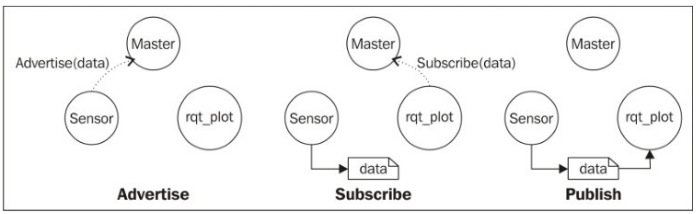
\includegraphics[scale=0.43]{imagens/rosmaster.png}\\
				{\footnotesize \textbf{Fonte:}}
			\end{center}
			\label{fig:master}
		\end{figure}
	\end{alertblock}
\end{frame}

% Slide COMPONENTES ROS PARAMETERS
%-----------------------------------------------------------------
\metroset{titleformat frame=smallcaps}
\begin{frame}{\textit{Robot Operating System-ROS}}
	\begin{alertblock}{Componentes ROS: Parâmetros ROS}
		\vspace{1cm}
		\begin{itemize}
			\setlength\itemsep{1.4em}
			\item São variáveis globais que podem ser usadas por nós.
			\item O principal objetivo dos parâmetros é fornecer ao sistema a capacidade de	se adaptar a cenários distintos de maneira ágil.
			\item Os parâmetros são	criados com valores padrões
		\end{itemize}
	\end{alertblock}
\end{frame}



%=================================================================
% PARTE II: DESENVOLVIMENTO
%=================================================================
\section{Parte II: Desenvolvimento}

%*****************************************************************
% CAPITULO I ARQUITETURA
%*****************************************************************

% Slide COMPONENTES DO SISTEMA
%-----------------------------------------------------------------
\begin{frame}{Arquitetura do Sistema}
    \begin{alertblock}{}
		%\vspace{0.4cm}
        \metroset{block=fill}
        \begin{block}{Programação de rede:}
            \begin{itemize}
                \item Efetuar programação de sockets e bibliotecas específicas para trabalho em redes.
            \end{itemize}
        \end{block}
		\vspace{0.25cm}
        \begin{block}{Aplicação ROS:}
            \begin{itemize}
                \item Desenvolver um pacote ROS para disponibilizar os dados recebidos dos outros pacotes ROS do sistema para o SoC.
            \end{itemize}
        \end{block}
		\vspace{0.25cm}
		\begin{block}{Aplicação HPS-SoC:}
            \begin{itemize}
                \item Estabelecer a comunicação entre a interface de rede da placa E10-nano através de	um programa executado no HPS do SoC, mantendo uma conexão entre o HPS e o FPGA.
            \end{itemize}
        \end{block}
    \end{alertblock}
\end{frame}


% Slide CLIENTE-SERVIDOR
%-----------------------------------------------------------------
\begin{frame}{Arquitetura do Sistema}
    \begin{alertblock}{Modelo cliente-servidor}
		\vspace{0.2cm}
		\begin{itemize}
			\item A comunicação entre o \textit{host} e a placa DE10-nano através de uma rede gigabit.
			\item Possui estrutura que permite dividir o esforço computacional.
			\item Contribui de forma significativa para a modularização do sistema.
		\end{itemize}
		\begin{figure}[h]
			%\caption{ROS Master}
			\begin{center}
				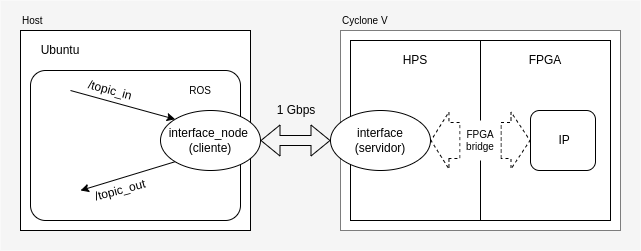
\includegraphics[scale=0.42]{imagens/arquitetura_geral.png}\\
				{\footnotesize \textbf{Fonte:}}
			\end{center}
			\label{fig:arquitetura}
		\end{figure}
	\end{alertblock}
\end{frame}


% Slide CLIENTE-SERVIDOR
%-----------------------------------------------------------------
\metroset{titleformat frame=smallcaps}
\begin{frame}{Arquitetura do Sistema}
	\begin{alertblock}{Biblioteca de comunicação - libinterfacesocket}
		\vspace{0.2cm}
	    \begin{itemize}
			\setlength\itemsep{0.7em}
	        \item Para manter o padrão do desenvolvimentos dos códigos tanto do cliente quanto do servidor.
	        \item Classe foi desenvolvida como um módulo à parte e compilada como uma biblioteca estática.
	        \item Alterações ou correções de erros, sem alterações nos códigos do servidor ou do cliente.
	        \item Programação da biblioteca foi realizada com base em sockets.
	        \item A programação de sockets em C++ possibilita um alto nível de otimização da comunicação.
	        \item Código fonte disponível no Github.
	    \end{itemize}
	\end{alertblock}
\end{frame}

%*****************************************************************
% CAPITULO II CLIENTE
%*****************************************************************

% Slide PACOTE ROS
%-----------------------------------------------------------------
\begin{frame}{Pacote ROS (cliente)}
    \begin{alertblock}{}
		%\vspace{0.2cm}
		\begin{columns}
			\column{.55\textwidth}
			%\begin{justify}
				No desenvolvimento de aplicações com ROS deve ser respeitada a estrutura de
				diretórios de um pacote ROS, portanto o desenvolvimento do cliente deve lever em consideração essa estrutura.
			%\end{justify}
			\column{.45\textwidth}
			\begin{figure}[h]
				%\caption{ROS Master}
				\begin{center}
					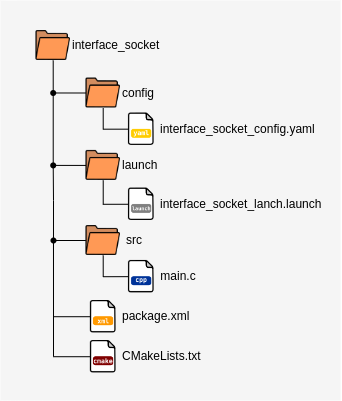
\includegraphics[scale=0.4]{imagens/rospackage.png}\\
					{\footnotesize \textbf{Fonte:}}
				\end{center}
				\label{fig:pkg}
			\end{figure}
		\end{columns}
	\end{alertblock}
\end{frame}

% Slide APLICAÇÃO CLIENTE
%-----------------------------------------------------------------
\metroset{titleformat frame=smallcaps}
\begin{frame}{Pacote ROS (cliente)}
	\begin{alertblock}{}
		%\vspace{0.2cm}
		\begin{columns}
			%\hspace{0.1cm}
			\column{.55\textwidth}
			\begin{itemize}
				\setlength\itemsep{0.6em}
				\item Configurações iniciais e leitura dos parâmetro.
				\item Cria o publisher e subscriber.
				\item Calback ler um tópico enviado por outro nó ROS.
				\item Faz o tratamento dos dados recebidos e os envia a SoC.
				\item Recebe dados do SoC e montar mensagem ROS para ser publicado em um tópico
			\end{itemize}
			\column{.45\textwidth}
			\begin{figure}[h]
				%\caption{ROS Master}
				\begin{center}
					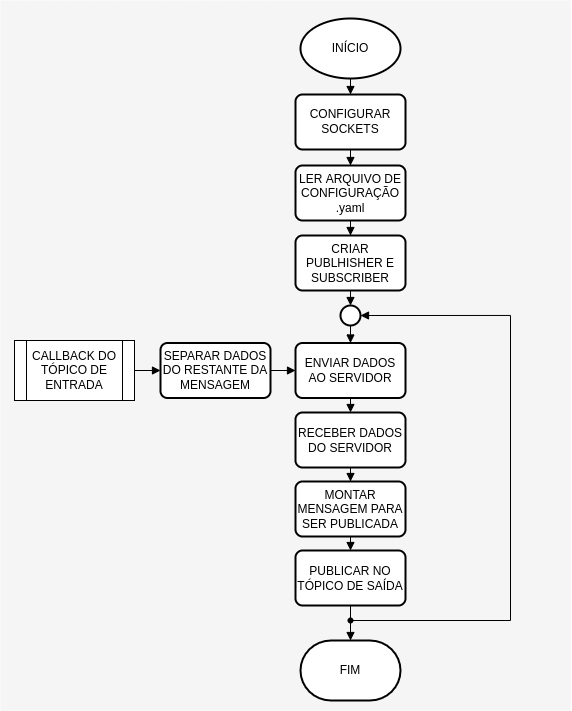
\includegraphics[scale=0.24]{imagens/fluxogramaCliente.png}\\
					{\footnotesize \textbf{Fonte:}}
				\end{center}
				\label{fig:cliente}
			\end{figure}
		\end{columns}
	\end{alertblock}
\end{frame}

%*****************************************************************
% CAPITULO III SERVIDOR
%*****************************************************************

% Slide SERVIDOR
%-----------------------------------------------------------------
\metroset{titleformat frame=smallcaps}
\begin{frame}{Servidor}
	\begin{alertblock}{}
		\vspace{0.2cm}
	    \begin{justify}
			Neste trabalho o programa servidor disponibiliza ao cliente a interface com o FPGA presente no SoC. Assim, ao receber o pedido do cliente, o servidor deve ser capaz de enviar os dados vindos do cliente à unidade de processamento embarcada no FPGA e em seguida devolver esses dados já processados ao cliente
	    \end{justify}
	\end{alertblock}
\end{frame}

% Slide BOOT
%-----------------------------------------------------------------
\begin{frame}{Arquitetura do Sistema}
    \begin{alertblock}{Processo de BOOT}
		\vspace{0.2cm}
		% \begin{itemize}
		% 	\item A comunicação entre o \textit{host} e a placa DE10-nano através de uma rede gigabit.
		% 	\item Possui estrutura que permite dividir o esforço computacional.
		% 	\item Contribui de forma significativa para a modularização do sistema.
		% \end{itemize}
		\begin{figure}[h]
			%\caption{ROS Master}
			\begin{center}
				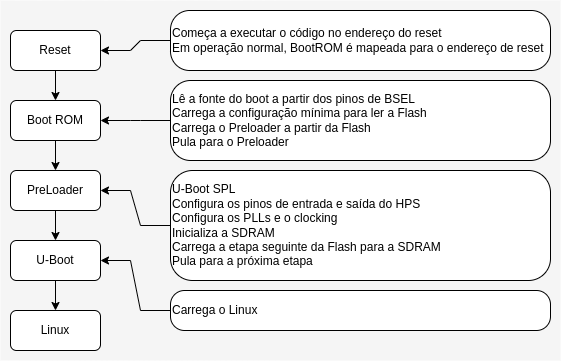
\includegraphics[scale=0.45]{imagens/embeddedLinux.png}\\
				{\footnotesize \textbf{Fonte:}}
			\end{center}
			\label{fig:boot}
		\end{figure}
	\end{alertblock}
\end{frame}

% Slide RSYOCTO
%-----------------------------------------------------------------
\metroset{titleformat frame=smallcaps}
\begin{frame}{Servidor}
	\begin{alertblock}{Distribuição Linux rsyocto}
		\vspace{0.1cm}
		\begin{justify}
			O rsyocto foi a distribuição distribuição linux escolhida, desenvolvida exclusivamente para SoCs da Intel com FPGA integrado. Algumas das suas caracteristicas são:
		\end{justify}
		\begin{itemize}
			%\setlength\itemsep{0.6em}
			\item Linux Kernel 5.11.
			\item Acesso total ao Dual-Core ARM (ARMv7-A) Cortex-A9.
			\item Configuração da malha FPGA durante o boot e com comandos Linux simples.
			\item Todas as interfaces entre o HPS e o FPGA estão habilitadas e prontas para uso.
			\item Ferramentas para interagir com a malha do FPGA a partir das ARM AXI HPS-
			toFPGA bridges.
		\end{itemize}
	\end{alertblock}
\end{frame}

% Slide INTERFACE SOCKET SERVER
%-----------------------------------------------------------------
\begin{frame}{Servidor}
    \begin{alertblock}{Servidor: Interface socket server}
		\vspace{0.3cm}
		\begin{itemize}
			\item Baixar, compilar e intalar a libinterfacesocket no linux embarcado.
			\item Mantém uma porta aberta esperando a conexão com o cliente.
			\item Dados recebidos do cliente são enviados para serem processados pelo FPGA e em seguida devolvidos ao cliente.
			\item O acesso do servidor ao FPGA é feito através de mapeamento de endereços do
			linux.
		\end{itemize}
		\begin{figure}[h]
			%\caption{ROS Master}
			\begin{center}
				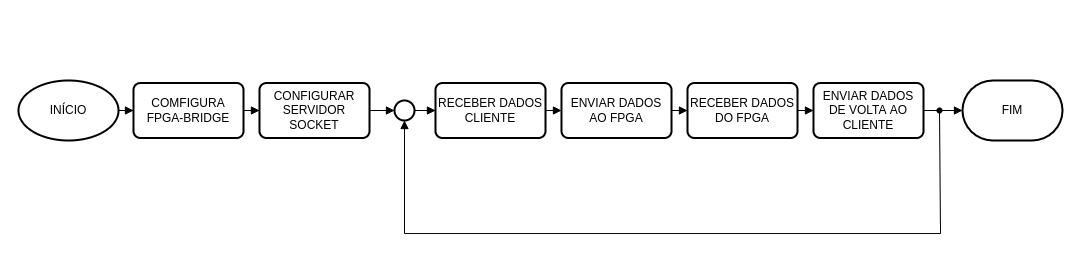
\includegraphics[scale=0.28]{imagens/fluxogramaServidor.png}\\
				{\footnotesize \textbf{Fonte:}}
			\end{center}
			\label{fig:servidor}
		\end{figure}
	\end{alertblock}
\end{frame}

% Slide SERVIDOR
%-----------------------------------------------------------------
\begin{frame}{Servidor}
    \begin{alertblock}{Servidor: Interface socket server}
		\vspace{0.2cm}
		\begin{figure}[h]
			%\caption{ROS Master}
			\begin{center}
				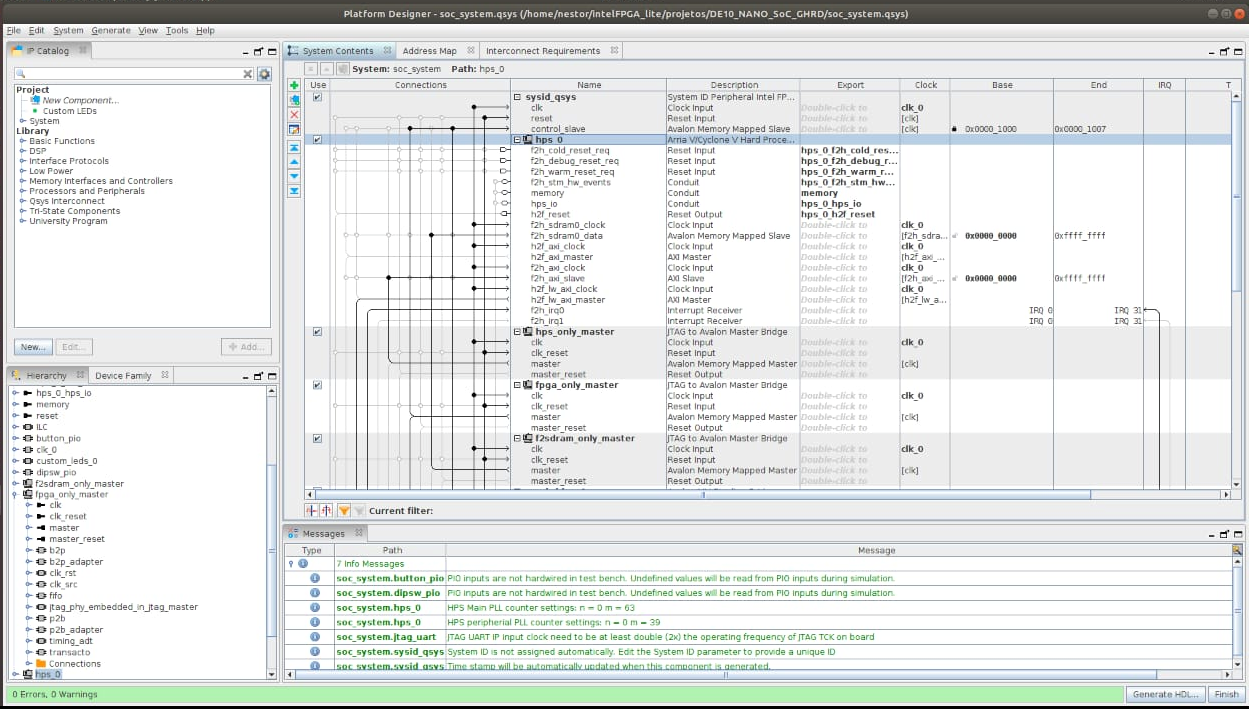
\includegraphics[scale=0.24]{imagens/Platiform.png}\\
				{\footnotesize \textbf{Fonte:}}
			\end{center}
			\label{fig:platform}
		\end{figure}
	\end{alertblock}
\end{frame}

% Slide SERVIDOR
%-----------------------------------------------------------------
% \metroset{titleformat frame=smallcaps}
% \begin{frame}{Servidor}
% 	\begin{alertblock}{}
% 		\vspace{0.2cm}
% 	    \begin{justify}
% 			Neste trabalho o programa servidor disponibiliza ao cliente a interface com o FPGA presente no SoC. Assim, ao receber o pedido do cliente, o servidor deve ser capaz de enviar os dados vindos do cliente à unidade de processamento embarcada no FPGA e em seguida devolver esses dados já processados ao cliente
% 	    \end{justify}
% 	\end{alertblock}
% \end{frame}


%=================================================================
% PARTE III:RESULTADOS
%=================================================================
\section{Parte III: Resultados}


% Slide RESULTADOS
%-----------------------------------------------------------------
\metroset{titleformat frame=smallcaps}
\begin{frame}{Resultados Alcançados}
    \begin{alertblock}{}
		%\vspace{0.4cm}
		\begin{justify}
			Foram idealizados dois ensaios: o primeiro com o objetivo de testar o fluxo completo de troca de dados entre um nó ROS e o FPGA; o segundo ensaio teve o objetivo de testar um fluxo grande de dados trafegando entre o ROS e o SoC.
		\end{justify}
        %\metroset{block=fill}
        \begin{block}{Teste Comunicação:}
            \begin{itemize}
                \item verificar a comunicação completa entre o nó ROS e um IP sendo executado no FPGA.
                \item foi projetado um circuito simples que	calcula o dobro de um número.
            \end{itemize}
        \end{block}
		\vspace{0.25cm}
        \begin{block}{Teste Rede:}
            \begin{itemize}
                \item testar a sobrecarga de dados na rede e avaliar o seu comportamento.
                \item \textit{Stream} de vídeo com resolução de 1280x720 em 15 fps.
            \end{itemize}
        \end{block}
    \end{alertblock}
\end{frame}

% Slide RESULTADOS GRÁFICOS
%-----------------------------------------------------------------
\metroset{titleformat frame=smallcaps}
\begin{frame}{Resultados Alcançados}
	%\begin{alertblock}{}
			\begin{figure}[h]
				%\caption{ROS Master}
				\begin{center}
					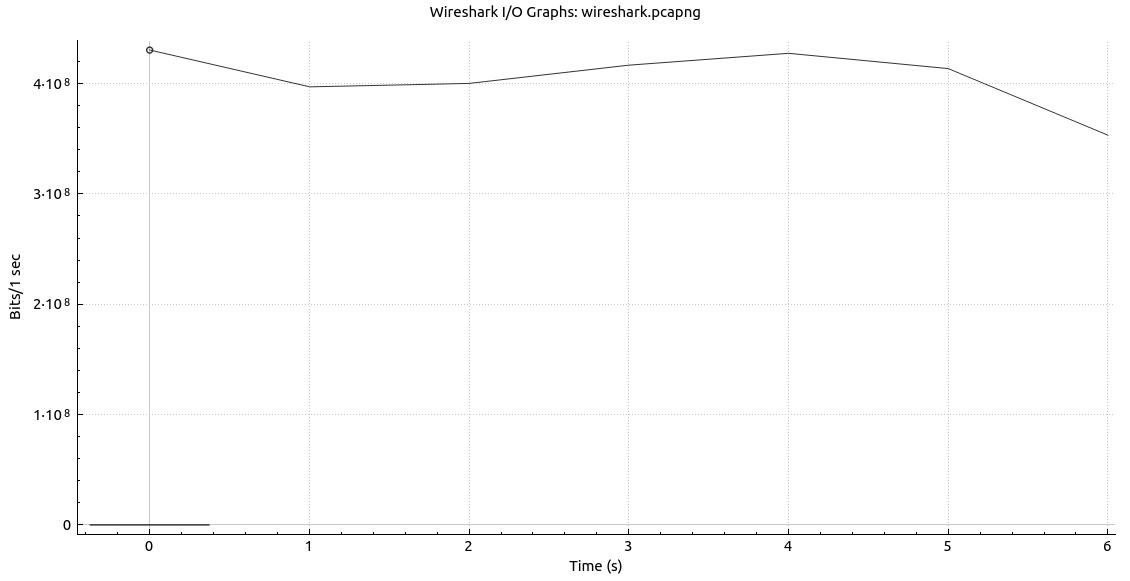
\includegraphics[scale=0.24]{imagens/speed.jpg}\\
					% {\footnotesize \textbf{Fonte:}}
				\end{center}
				\label{fig:speed}
			\end{figure}

			\begin{figure}[h]
				%\caption{ROS Master}
				\begin{center}
					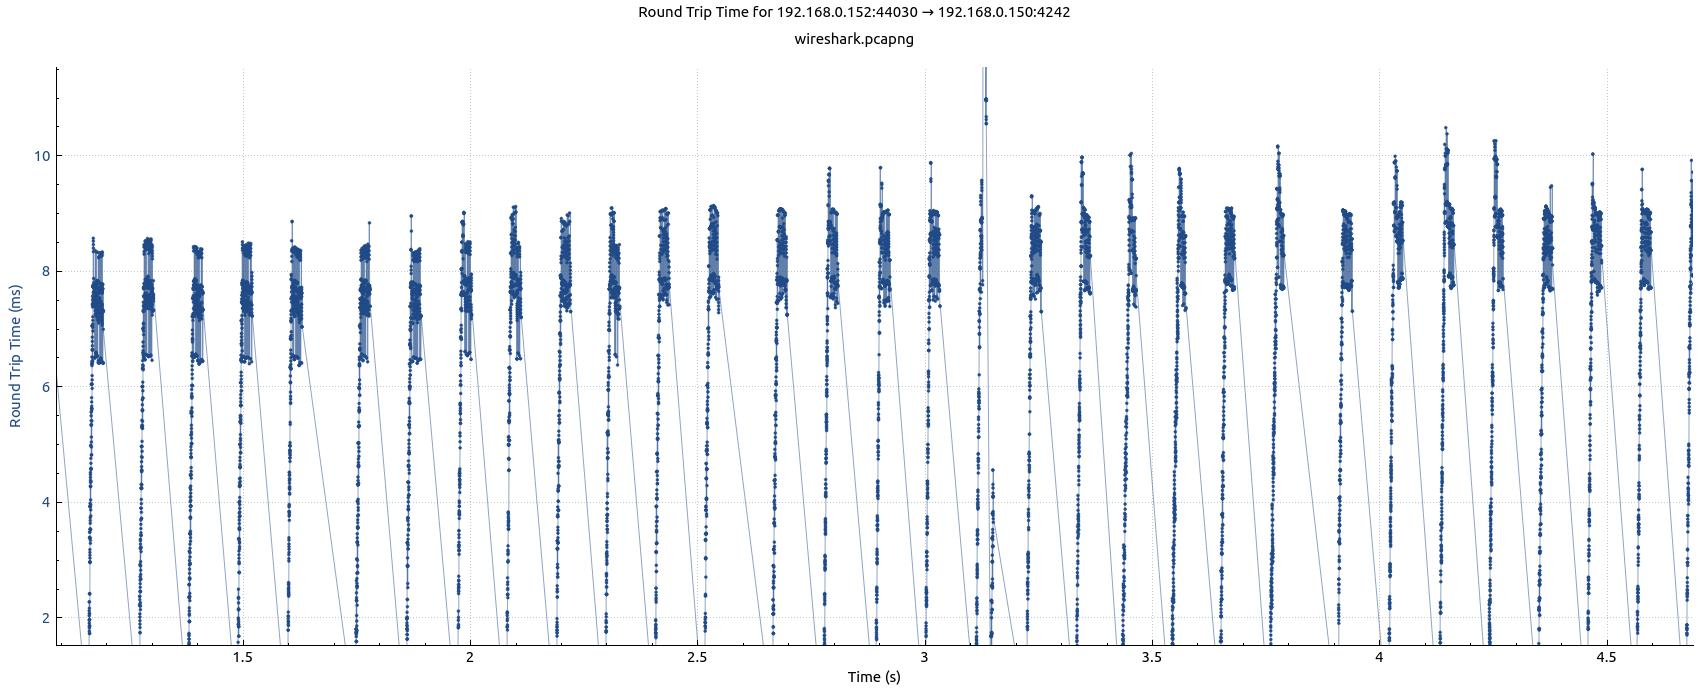
\includegraphics[scale=0.19]{imagens/delay.jpg}\\
					{\footnotesize \textbf{Fonte:}}
				\end{center}
				\label{fig:delay}
			\end{figure}

	%\end{alertblock}
\end{frame}

% Slide CONCLUSÃO
%-----------------------------------------------------------------
\metroset{titleformat frame=smallcaps}
\begin{frame}{Conclusão}
	\begin{alertblock}{}
		\vspace{0.2cm}
		\begin{justify}
			Os resultados alcançados para os dois ensaios foram considerados satisfatórios, apesar de, na transferência das imagens, ter sido observado um pequeno delay, menor do que 10 ms.
		\end{justify}
		\vspace{1cm}
		{\small Trabalho publicado no 28º IBERCHIP Workshop, promovido pela IEEE Circuits and Systems Society - CASS, Santiago no Chile, 2022.}
	\end{alertblock}
\end{frame}

% Slide TRABALHOS FUTUROS
%-----------------------------------------------------------------
% \metroset{titleformat frame=smallcaps}
% \begin{frame}{Estudos futuros}
% 	\begin{alertblock}{}
% 		\vspace{0.2cm}
% 	    \begin{justify}
% 			Neste trabalho o programa servidor disponibiliza ao cliente a interface com o FPGA presente no SoC. Assim, ao receber o pedido do cliente, o servidor deve ser capaz de enviar os dados vindos do cliente à unidade de processamento embarcada no FPGA e em seguida devolver esses dados já processados ao cliente
% 	    \end{justify}
% 	\end{alertblock}
% \end{frame}





% {\setbeamercolor{palette primary}{fg=black, bg=yellow}
% \begin{frame}[standout]
%   Questions?
% \end{frame}
% }


\begin{frame}[allowframebreaks]{Referencias}
  \bibliography{demo}
  %\bibliographystyle{abbrv}
  \bibliographystyle{acm}
\end{frame}

\end{document}



%\begin{frame}{Blocks}
%  Three different block environments are pre-defined and may be styled with an
%  optional background color.

%  \begin{columns}[T,onlytextwidth]
%    \column{0.5\textwidth}
%      \begin{block}{Default}
%        Block content.
%      \end{block}

%      \begin{alertblock}{Alert}
%        Block content.
%      \end{alertblock}

%      \begin{exampleblock}{Example}
%        Block content.
%      \end{exampleblock}

%    \column{0.5\textwidth}

%      \metroset{block=fill}

%      \begin{block}{Default}
%        Block content.
%      \end{block}

%      \begin{alertblock}{Alert}
%        Block content.
%      \end{alertblock}

%      \begin{exampleblock}{Example}
%        Block content.
%      \end{exampleblock}
%
%  \end{columns}
%\end{frame}




%{%
%\setbeamertemplate{frame footer}{My custom footer}
%\begin{frame}[fragile]{Frame footer}
%    \themename defines a custom beamer template to add a text to the footer. It can be set via
%    \begin{verbatim}\setbeamertemplate{frame footer}{My custom footer}\end{verbatim}
%\end{frame}
%}



% \metroset{titleformat frame=smallcaps}
% \begin{frame}{Cronograma}
% 	\begin{alertblock}{Metas físicas}
%         \begin{enumerate}[1.]
%         	\item Levantamento bibliográfico sobre os assuntos mais relevantes do projeto: ROS, Nios II, Verilog HDL, RTOS, TCP/IP Stack, Sockets.
%         	\item Estudo detalhado do protocolo de comunicação entre os nós no ROS.
%         	\item Desenvolvimento do sistema base do Nios II no Platform Designer.
%         	\item Implementação do RTOS no sistema base.
%         	\item Testes de comunicação TCP/IP entre o PC e o sistema embarcado no FPGA.
%         	\item Desenvolvimento de uma aplicação de processamento de vídeo em FPGA.
%         	\item Avaliação do desempenho do sistema proposto.
%         	\item Elaboração da dissertação e publicação dos resultados.
%         \end{enumerate}
% 	\end{alertblock}
% \end{frame}



% \metroset{titleformat frame=smallcaps}
% \begin{frame}{Cronograma}

%     \begin{table}[h]
%     	\centering

%     	\vspace{0.2cm}
%     	\begin{tabular}{c|cccccccccccc}
%     		\toprule
%     		 & \multicolumn{12}{c}{{\tiny Meses}}\\ 
%     		{\tiny Metas} & {\tiny 1} & {\tiny 2} & {\tiny 3} & {\tiny 4} & {\tiny 5} & {\tiny 6} & {\tiny 7} & {\tiny 8} & {\tiny 9} & {\tiny 10} & {\tiny 11} & {\tiny 12} \\ 
%     		\midrule  
%     		\midrule                           
%     		{\tiny Levantamento Bibliográfico}& $\circledast$ & & & & & & & & & & & \\
%     		\hline
%     		{\tiny Estudo protocolos ROS} & & $\circledast$ & $\circledast$ & $\circledast$ & $\circledast$ & $\circledast$ & & & & & &  \\
%     		\hline
%     		{\tiny Desenv. do Nios II} & & & $\circledast$ & $\circledast$ & & & & & & & &  \\
%     		\hline
%     		{\tiny Implementação } {\tiny do RTOS} & & & & $\circledast$ & $\circledast$ & $\circledast$ & & & & & &  \\
%     		\hline
%     		{\tiny Testes de Comunicação} & & & & & & $\circledast$ & $\circledast$ & $\circledast$ & & & &  \\
%     		\hline
%     		{\tiny Desenv. do coprocessador} & & & & & & & & $\circledast$ & $\circledast$ & $\circledast$ & $\circledast$ &  \\
%     		\hline
%     		{\tiny Avaliação do desempenho} & & & & & & & & & & $\circledast$ & $\circledast$ & $\circledast$ \\
%     		\hline
%     		{\tiny Elaboração da } {\tiny dissertação} & & & & & & $\circledast$ & $\circledast$ & $\circledast$ & $\circledast$ & $\circledast$ & $\circledast$ & $\circledast$\\
%     		\bottomrule 
    
%     	\end{tabular}
%     	\\
%     	\label{tab:crono}
%     \end{table}
% \end{frame}